Visualize the hyperboloid of one sheet defined by

\begin{align*}
    x^2/a^2 + y^2/b^2 - z^2/c^2 - 1 = 0
\end{align*}

for different values $a$, $b$, $c$. What features do $a$, $b$, and $c$ control?

\begin{solution}\
\begin{lstlisting}
a = 1.5;
b = 1;
c = 1;
[x,y,z] = meshgrid(linspace(-10,10,100),linspace(-10,10,100),linspace(-10,10,100));
f = x.^2/a^2 + y.^2/b^2 - z.^2/c^2 - 1;
isosurface(x, y, z, f, 0)
\end{lstlisting}

\begin{center}
    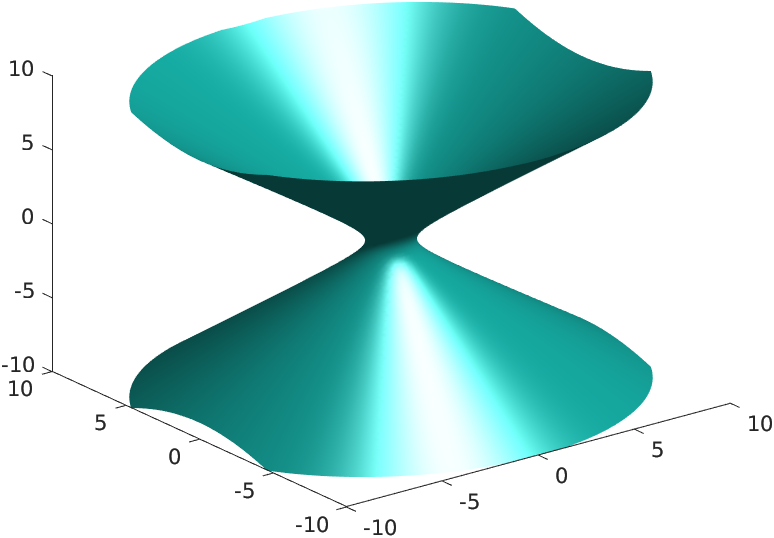
\includegraphics[width=0.5\textwidth]{img/e14p1.png}
\end{center}

$a$, $b$, and $c$ control the stretching in the $x$, $y$, and $z$ directions, respectively.
\end{solution}